\begin{frame}[allowframebreaks]{Clustering - K-means}
\begin{columns}
    \begin{column}{0.45\textwidth}
        Groups data into $K$ clusters that  satisfy two properties.
        \vspace{0.8em}
        \begin{enumerate}
            \setlength{\itemsep}{0.5em}
            \item Each observation belongs to at least one of the $K$ clusters.
            \item Clusters are non-overlapping.  No observation belongs to more  than one cluster.
        \end{itemize}
    \end{column}
    \begin{column}{0.55\textwidth}
        \begin{figure}
            \centering
            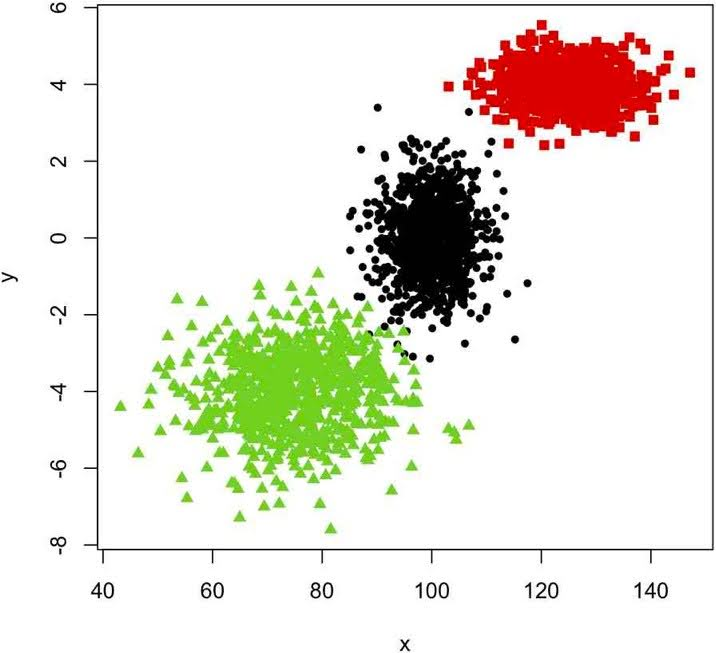
\includegraphics[width=0.95\textwidth,keepaspectratio]{images/dul/kmeans/k-means-example-1.jpg}
            \caption{Clusters.}
        \end{figure}
    \end{column}
\end{columns}

\framebreak

\begin{columns}
    \begin{column}{0.45\textwidth}
    A good clustering is one for which the \textit{within-cluster variation} is as small as possible.

    \vspace{1em}

    Denote each cluster by $C_k$, and let $W(C_k)$ be a measure of the within-cluster variation.

    \vspace{1em}

    K-means aims to solve the following optimization problem:

    \vspace{0.5em}

    \begin{equation}
        \operatorname*{minimise}_{C_1, \ldots, C_k} \left\{ \sum_{k=1}^{K} W(C_k) \right\}
    \end{equation}

    \end{column}
    \begin{column}{0.55\textwidth}
        \begin{figure}
            \centering
            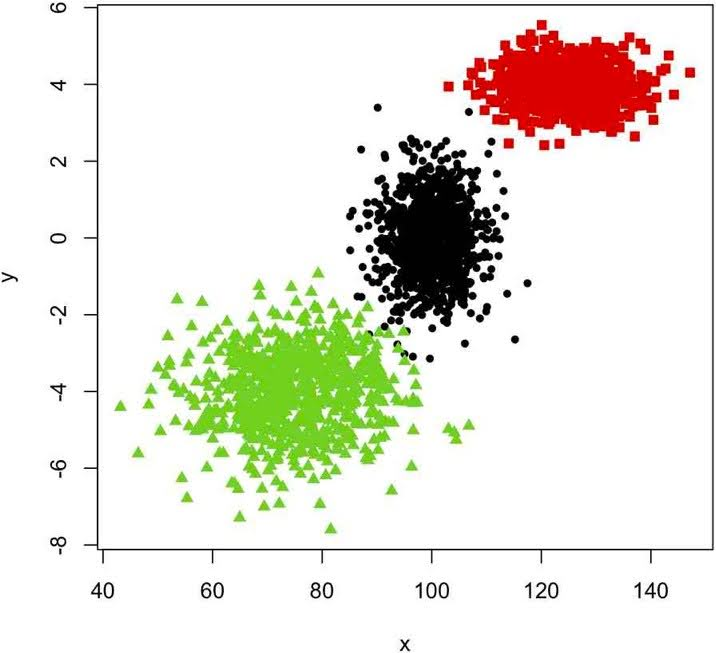
\includegraphics[width=0.95\textwidth,keepaspectratio]{images/dul/kmeans/k-means-example-1.jpg}
            \caption{Clusters.}
        \end{figure}
    \end{column}
\end{columns}

\framebreak

\begin{block}{}
    How to measure within-cluster variation? 

    \vspace{0.5em}

    The most common choice is squared Euclidean distance:
        \begin{equation}
            W(C_k) = \frac{1}{|C_k|} \sum_{i, i' \in C_k} \sum_{j=1}^{p} (x_{ij} - x_{i'j})^2
        \end{equation}
    
        where $|C_k|$ is the number of points in cluster $C_k$ and $x_{ij}$ is the $j^{th}$ feature of the $i^{th}$ point.
    
    \vspace{0.5em}
    
    Which means overall we solve:
        \begin{equation}
            \operatorname*{minimise}_{C_1, \ldots, C_k} \left\{ \sum_{k=1}^{K} \frac{1}{|C_k|} \sum_{i, i' \in C_k} \sum_{j=1}^{p} (x_{ij} - x_{i'j})^2 \right\}
        \end{equation}
\end{block}

\framebreak

\begin{itemize}
    \setlength{\itemsep}{0.5em}
    \item It turns out that this optimization problem is difficult to solve, as it is  discrete and there are nearly $K^n$	ways to split $n$ samples into $K$ clusters.
    \item In practice, use an iterative algorithm that finds a local minimum to this  optimization.
\end{itemize}

\framebreak

%pseudo code
\begin{algorithm}[H]
\caption{K-means Clustering Algorithm}
\KwIn{Dataset $D = \{x_1, x_2, \dots, x_n\}$, number of clusters $k$}
\KwOut{Cluster assignments for each data point}

\vspace{0.8em}

\textbf{Initialization:} Randomly initialize $k$ cluster centroids or seeds\;

\vspace{0.8em}

\textbf{Repeat until convergence:}
\begin{itemize}
    \item \textbf{Assignment Step:} Assign each data point $x_i$ to the nearest cluster based on a distance metric\;
    \vspace{0.5em}
    \item \textbf{Update Step:} Recompute cluster centroids using current assignments\;
    \vspace{0.5em}
    \item \textbf{Convergence Check:} Check if cluster assignments have changed or if centroids have stabilized\;
\end{itemize}

\vspace{0.8em}

\textbf{Return:} Final cluster assignments and centroids\;
\vspace{0.8em}

\end{algorithm}

\framebreak

\begin{center}
    Watch the K-means clustering algorithm in action:

    \vspace{1em}

    % \fetchconvertimageonly{https://i.ytimg.com/an_webp/2lZZ_FzlIJY/mqdefault_6s.webp?du=3000&sqp=CJLBvMEG&rs=AOn4CLBgJ_07yNkEYOFCkUraCWAH8Zmrsg}{images/thumbnails/k-means-youtube-thumbnail.png}
    \href{https://www.youtube.com/watch?v=2lZZ_FzlIJY}{%
    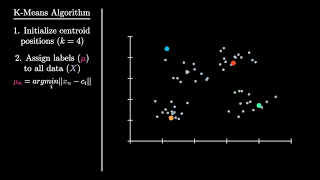
\includegraphics[width=0.95\textwidth,keepaspectratio]{images/thumbnails/k-means-youtube-thumbnail-0.png}
    }
    % \animategraphics[loop,controls,width=0.65\linewidth]{2}{images/gif_frames/k-mean-}{001}{014}
    % \includeGIF{images/k-mean-animation.gif}{k-mean}{0.95\linewidth}{12}
\end{center}

\framebreak

\begin{columns}
    \begin{column}{0.45\textwidth}
        \begin{enumerate}
            \setlength{\itemsep}{1em}
            \item It can be shown that the value of  the objective function will never  increase at each iteration of $k$-means.
            \item Since the algorithm finds local  minima, however, it will result in  different clusters with different  initializations.
        \end{itemize}
    \end{column}
    \begin{column}{0.55\textwidth}
        \begin{figure}
            \centering
            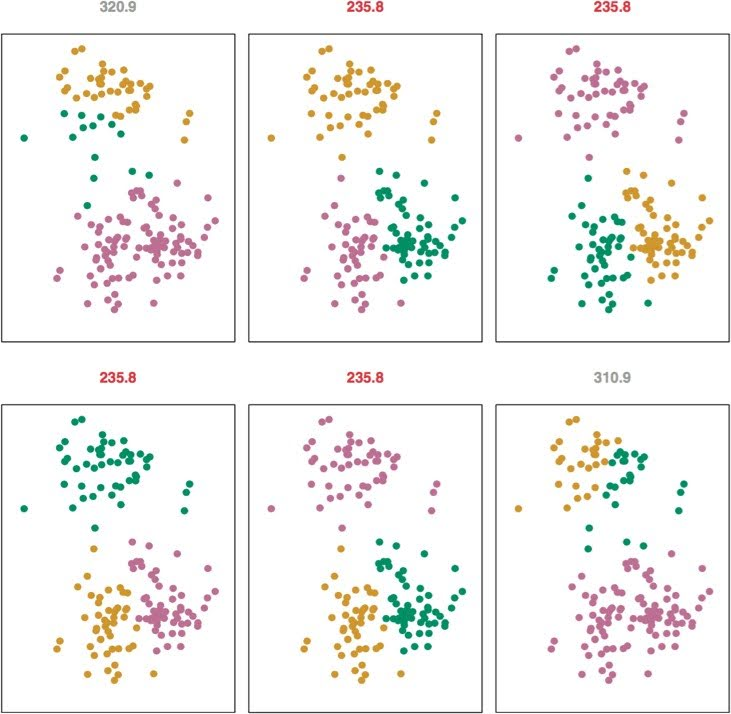
\includegraphics[width=\textwidth,keepaspectratio]{images/dul/kmeans/k-mean-different-init.jpg}
            \caption{Different initializations of K-means.}
        \end{figure}
    \end{column}
\end{columns}

\end{frame}

\begin{frame}[allowframebreaks]{K-means - Pros and Cons}
\begin{columns}
    \begin{column}{0.45\textwidth}
        \textbf{Pros}
        \begin{itemize}
            \setlength{\itemsep}{1em}
            \item Simple and easy to implement
            \item Efficient for large datasets
            \item Works well with spherical clusters
            \item Scalable to large datasets
        \end{itemize}
    \end{column}
    \begin{column}{0.55\textwidth}
        \textbf{Cons}
        \begin{itemize}
            \setlength{\itemsep}{1em}
            \item Not robust to data perturbations and different initializations
            \item Sensitive to initial centroid placement
            \item Assumes spherical clusters
            \item Requires specifying the number '$K$' of clusters in advance
            \item Sensitive to outliers
            \item May converge to local minima
            \item Not suitable for non-convex shapes
        \end{itemize}
    \end{column}
\end{columns}
\end{frame}